\documentclass[handout,nooutcomes,noauthor,hints]{ximera}

\graphicspath{  
{./}
{./whoAreYou/}
{./drawingWithTheTurtle/}
{./bisectionMethod/}
{./circles/}
{./anglesAndRightTriangles/}
{./lawOfSines/}
{./lawOfCosines/}
{./plotter/}
{./staircases/}
{./pitch/}
{./qualityControl/}
{./symmetry/}
{./nGonBlock/}
}


%% page layout
\usepackage[cm,headings]{fullpage}
\raggedright
\setlength\headheight{13.6pt}


%% fonts
\usepackage{euler}

\usepackage{FiraMono}
\renewcommand\familydefault{\ttdefault} 
\usepackage[defaultmathsizes]{mathastext}
\usepackage[htt]{hyphenat}

\usepackage[T1]{fontenc}
\usepackage[scaled=1]{FiraSans}

%\usepackage{wedn}
\usepackage{pbsi} %% Answer font


\usepackage{cancel} %% strike through in pitch/pitch.tex


%% \usepackage{ulem} %% 
%% \renewcommand{\ULthickness}{2pt}% changes underline thickness

\tikzset{>=stealth}

\usepackage{adjustbox}

\setcounter{titlenumber}{-1}

%% journal style
\makeatletter
\newcommand\journalstyle{%
  \def\activitystyle{activity-chapter}
  \def\maketitle{%
    \addtocounter{titlenumber}{1}%
                {\flushleft\small\sffamily\bfseries\@pretitle\par\vspace{-1.5em}}%
                {\flushleft\LARGE\sffamily\bfseries\thetitlenumber\hspace{1em}\@title \par }%
                {\vskip .6em\noindent\textit\theabstract\setcounter{question}{0}\setcounter{sectiontitlenumber}{0}}%
                    \par\vspace{2em}
                    \phantomsection\addcontentsline{toc}{section}{\thetitlenumber\hspace{1em}\textbf{\@title}}%
                     }}
\makeatother



%% thm like environments
\let\question\relax
\let\endquestion\relax

\newtheoremstyle{QuestionStyle}{\topsep}{\topsep}%%% space between body and thm
		{}                      %%% Thm body font
		{}                              %%% Indent amount (empty = no indent)
		{\bfseries}            %%% Thm head font
		{)}                              %%% Punctuation after thm head
		{ }                           %%% Space after thm head
		{\thmnumber{#2}\thmnote{ \bfseries(#3)}}%%% Thm head spec
\theoremstyle{QuestionStyle}
\newtheorem{question}{}



\let\freeResponse\relax
\let\endfreeResponse\relax

%% \newtheoremstyle{ResponseStyle}{\topsep}{\topsep}%%% space between body and thm
%% 		{\wedn\bfseries}                      %%% Thm body font
%% 		{}                              %%% Indent amount (empty = no indent)
%% 		{\wedn\bfseries}            %%% Thm head font
%% 		{}                              %%% Punctuation after thm head
%% 		{3ex}                           %%% Space after thm head
%% 		{\underline{\underline{\thmname{#1}}}}%%% Thm head spec
%% \theoremstyle{ResponseStyle}

\usepackage[tikz]{mdframed}
\mdfdefinestyle{ResponseStyle}{leftmargin=1cm,linecolor=black,roundcorner=5pt,
, font=\bsifamily,}%font=\wedn\bfseries\upshape,}


\ifhandout
\NewEnviron{freeResponse}{}
\else
%\newtheorem{freeResponse}{Response:}
\newenvironment{freeResponse}{\begin{mdframed}[style=ResponseStyle]}{\end{mdframed}}
\fi



%% attempting to automate outcomes.

%% \newwrite\outcomefile
%%   \immediate\openout\outcomefile=\jobname.oc
%% \renewcommand{\outcome}[1]{\edef\theoutcomes{\theoutcomes #1~}%
%% \immediate\write\outcomefile{\unexpanded{\outcome}{#1}}}

%% \newcommand{\outcomelist}{\begin{itemize}\theoutcomes\end{itemize}}

%% \NewEnviron{listOutcomes}{\small\sffamily
%% After answering the following questions, students should be able to:
%% \begin{itemize}
%% \BODY
%% \end{itemize}
%% }
\usepackage[tikz]{mdframed}
\mdfdefinestyle{OutcomeStyle}{leftmargin=2cm,rightmargin=2cm,linecolor=black,roundcorner=5pt,
, font=\small\sffamily,}%font=\wedn\bfseries\upshape,}
\newenvironment{listOutcomes}{\begin{mdframed}[style=OutcomeStyle]After answering the following questions, students should be able to:\begin{itemize}}{\end{itemize}\end{mdframed}}



%% my commands

\newcommand{\snap}{{\bfseries\itshape\textsf{Snap!}}}
\newcommand{\flavor}{\link[\snap]{https://snap.berkeley.edu/}}
\newcommand{\mooculus}{\textsf{\textbf{MOOC}\textnormal{\textsf{ULUS}}}}


\usepackage{tkz-euclide}
\tikzstyle geometryDiagrams=[rounded corners=.5pt,ultra thick,color=black]
\colorlet{penColor}{black} % Color of a curve in a plot



\ifhandout\newcommand{\mynewpage}{\newpage}\else\newcommand{\mynewpage}{}\fi


\title{Formulas galore}

\author{Bart Snapp}

\begin{document}
\begin{abstract}
We make estimates using basic formulas and determine what is, and is
not, a reasonable estimate.
\end{abstract}
\maketitle

\begin{listOutcomes}
\item Distinguish between reasonable and unreasonable estimates.
\item Determine a reasonable estimate before preforming a calculation.
\item Apply basic geometric formulas.
\end{listOutcomes}

Here are a bunch of formulas Dr.\ Snapp found on the internet at this site
\begin{center}
  \textit{https://sites.google.com/site/standardbasicengineering/home/useful-formula-for-finding-area-volume-of-solid-figures}
\end{center}
\begin{center}
  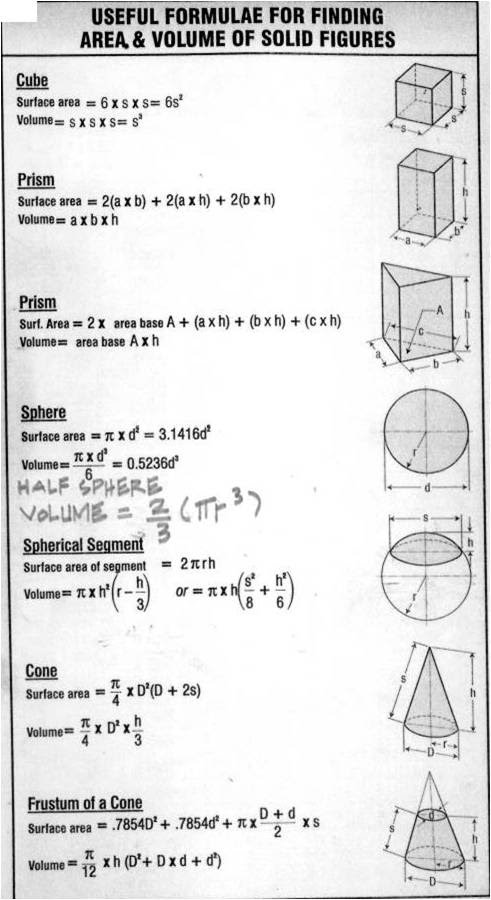
\includegraphics[width=.3\textwidth]{photoFormula1.jpg} \qquad 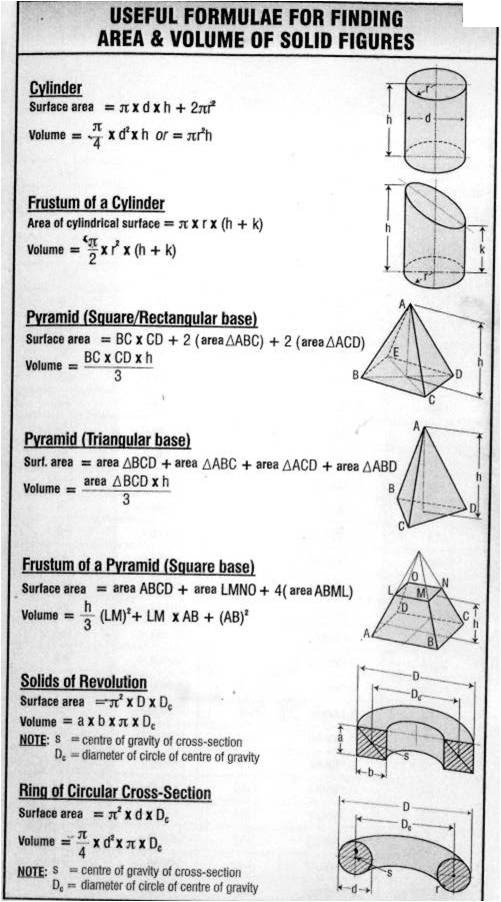
\includegraphics[width=.3\textwidth]{photoFormula2.jpg}
\end{center}

Let's think about some questions. 


\mynewpage




\begin{question} \label{FG1:1}
  Consider the \link[\textit{Ericsson Globe}]{https://en.wikipedia.org/wiki/Ericsson_Globe}:
   \begin{center}
    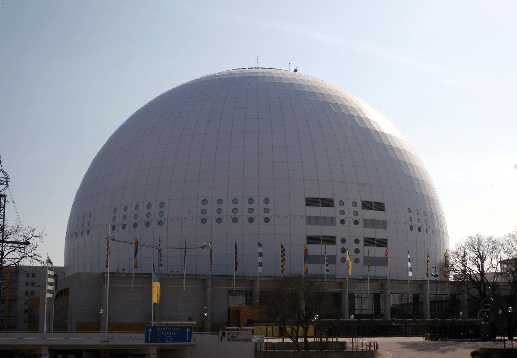
\includegraphics[width=.4\textwidth]{dome.png} %https://www.researchgate.net/figure/Example-of-a-hemispherical-dome-in-modern-civil-engineering-Stockholm-Globe-Arena-by_fig2_308655043
   \end{center}
   Assuming that this building has a diameter of $110$ meters and a
   height of $85$ meters.
   
   Use the formulas above to find the surface area
   and the volume of the \textit{Ericsson Globe}.
\begin{enumerate}
\item Estimate these values by finding the surface area and volume of
  a box with dimensions $100\times 100 \times 80$ meters. Show all work.
\item Compare the estimates above with estimates using the formulas
  found at the beginning of this activity. Explain your work and
  describe the percentage difference between the two estimates.
\end{enumerate}
\begin{freeResponse}
  \begin{enumerate}
  \item So if we use a box with dimensions $100\times 100 \times 80$ meters,
    we find the surface area is
    \[
    4\times 80 \times 100 = 32000~\text{square meters}
    \]
    and the volume is
    \[
    100\times 100 \times 80 = 800000~\text{cubic meters.}
    \]
    The box estimate is around $10\%$ greater than the formula
    estimate.
  \item If we use the formulas, the surface area will be
    \[
    2\pi rh
    \]
    where $h= 110-85 = 25$ and $r= 110/2 = 55$, so
    \[
    110 \pi - 2\pi 55\cdot 25 \approx  29000~\text{square meters}.
    \]
    The volume will be
    \[
    \pi h^2 \left( r- \frac{h}{3}\right)
    \]
    so
    \[
    \pi \times 25^2 (55 - 25/3) \approx 92000 ~\text{cubic meters.}
    \]
    The box estimate is around $13\%$ smaller than the formula
    estimate.
  \end{enumerate}
\end{freeResponse}
   \end{question}
\mynewpage

 \begin{question}   Consider the \link[\textit{Luxor Las Vegas}]{https://en.wikipedia.org/wiki/Luxor_Las_Vegas}.  Assume that the (square) base of this building has a side length of
 $646$ feet and that the pyramid is $350$ feet tall:
  \begin{center}
    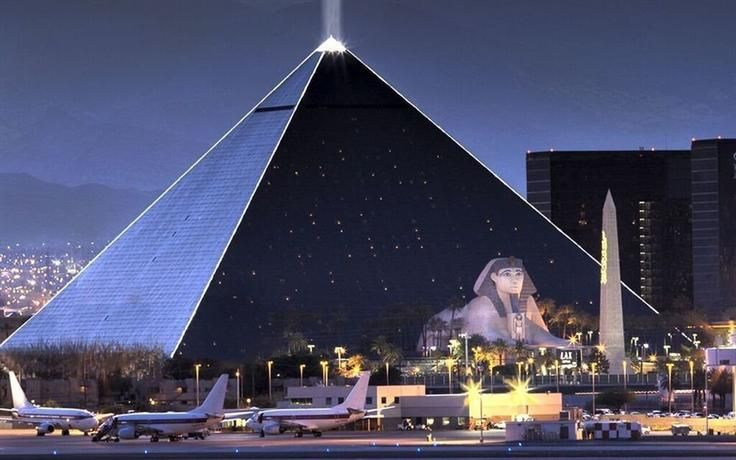
\includegraphics[width=.4\textwidth]{pyramid.jpg} 
  \end{center}

  \begin{enumerate}
  \item Which is \textbf{easier} to compute:
    \begin{itemize}
    \item the surface area (not including the bottom!) OR
    \item the volume
    \end{itemize}
    of the \textit{Luxor Las Vegas}?
    Explain why one computation is more difficult than the other.
    \item Compute the EASISER computation of the two above. Show all
      work.
  \end{enumerate}

   \begin{freeResponse}
    \begin{enumerate}
      \item The volume is MUCH EASIER to compute than the surface
        area. To compute the surface area, you have to compute the
        area of each face of the pyramid, this requires GEOMETRY.

      \item The volume is
        \[
        V = \frac{646\cdot 646\cdot 350}{3} \approx = 48686867 \text{ cubic feet}.
        \]
    \end{enumerate}
  \end{freeResponse}
\end{question}

\mynewpage

 \begin{question}%
    You ask six friends what the surface area of the top part of the
    \textit{Luxor Las Vegas} is. They give you six wrong answers, but
    you love them anyway, because they are your friends. Here are
    their answers:
    \begin{enumerate}
    \item $650$ square feet
    \item $6500$ square feet
    \item $65000$ square feet
    \item $650000$ square feet
    \item $6500000$ square feet
    \item $65000000$ square feet
    \end{enumerate}
      Which answer above is \textbf{closest} to the correct answer?
      Explain your reasoning.
      \begin{freeResponse}
        Answer $(iv)$ is correct, here's how I know. The pyramid has a
        base, and four more sides. The BIGGEST the surface area could
        be is
        \[
        4\cdot 350\cdot 646 = 904400.
        \]
        On the other hand, the area of the SMALLEST the surface area could be is
        the area of the base, or
        \[
        646\cdot 646 = 417316.
        \]
        Note, $417316 < 650000 <  904400$.        
      \end{freeResponse}
\end{question}





\end{document}
